\chapter{How to import FKB into OpenStreetMap}\label{ch:suggmethod}
%Proof of concept 
Looking at an import of FKB building data into the OSM database, how should the process be done? What are the challenges? Using previous chapters, this chapter will suggest an import method. It will also evaluate an existing conversion script and suggest improvements. At last it will evaluate how to import FKB buildings data to achieve a 3D representation of the buildings. 

\section{Micro-tasking method?}
% Går tilbake til metodene, hva kan vi lære i Norge hvor vi ikke har Mapbox. Norske FKB er bedre enn de man har importert i andre land
% Er dette beste metode?
%Hvordan dele opp i tasking områder? telle antall hus. 50-30-20 hus innenfor hver task? Dette er en utfordring, men er utenfor scopet til oppgaven. Komme med noen tanker rundt hvordan det kan løses. 
Chapter \ref{ch:importmethods} introduce three common import methods, one of them is the micro-tasking method. The micro-tasking method stand out as the best alternative when considering the three methods. Especially together with a micro-tasking tool like the OSM Tasking Manager. The method and tool together solve problems other import methods face. When using them it is not necessary to create a personal dev-website with a list of an import queue like Dave Hansen did during the Tiger import or creating a personal drive folder with the import files, like the OSM user tibnor did during N50 import. The micro-tasking method with the correct tool simplifies the import process.  

What is the correct tool? The micro-tasking method is of course dependent on a good tool that organize the tasks well. The tasks should be easy to select, to download, to comment on and to mark as resolved. Information about the import and how to complete the tasks should be available at all time and also be easy to understand. After some testing of the OSM Tasking Manager through this study, a safe assumption is that this tool solves the important parts mentioned above. Instead of having to read multiple import wiki pages, imports often have more than one information page, then follow email conversations about the import, ask which files to import next and after that having to find where the import files are located. The OSM  Tasking Manager gathers all these steps in one place, making it much easer for users to contribute on imports. 

The first challenge when using the micro-tasking method is dividing the dataset into smaller parts which give manageable sized tasks. Dividing the building datasets was a challenge in both the New York- and Los Angeles building import, introduced in section \ref{sec:importmicro}. Both solved this issue by dividing it into smaller parts using already defined subregions.*%Gir denne setningen mening?
 When considering the FKB building datasets, instead of dividing it into predefined regions, another alternative is to create subregions by counting buildings. The density of buildings varies between different areas in Norway. %The building density differs between city centers in the municipalities, and between regions outside the city center. 
 The counting approach would ensure that every task has a manageable size. The number of buildings within each task could be from 20-30 units. This number must off course be tested with a test import before a final decision is made. What's important is that finishing a task should not take more than a few hours maximum, but at the same time should not be too small either. Too small tasks will result in too many tasks. *%And? finish the sentence
 
Another challenge that will emerge in an import is overlapping buildings. There are already buildings on the OSM-map of Norway, for instance shown in figure \ref{fig:3Dekstrd} and \ref{fig:fruekirke2D}. These buildings are manually drawn and added by OSM users. Handling the conflicts according to the import guidelines is important. OpenStreetMap has no concept of layers, data on top of data will make it difficult for users to work in the standard OSM editors *.%kilde http://wiki.openstreetmap.org/wiki/Import/Guidelines
Overlapping layers needs to be merged. A reasonably safe assumption is that the building geometry is more accurate in FKB than in the manually drawn buildings. In JOSM there are a replace geometry tool. This tool replaces the geometry of the old building with the geometry of the new building while keeping all the tags and relations of the old one.*%Test, beholder den også den nye bygningens tags og relations?
When the LA team worked on a task, they had at least two layers in JOSM, one with current OSM data and the other with the imported data. Both layers are reviewed for possible conflicts. If data in OSM was better than the imported data, only tags are transferred. %https://github.com/osmlab/labuildings/blob/master/IMPORTING.md  
This process is probably a good solution when doing FKB building import, one should always consider the data already in OSM before importing new data.  

A huge advantage in both New York and Los Angeles building import was Mapbox. Having a company involved with professional staff who gets paid is challenging to replace. Luckily the tools created during both imports is open source, available at GitHub. Before implementing any new tool, the FKB building import team should look at already created tools. For instance, the LA-building team developed a plugin for JOSM called \textit{Auto-tools}. This tool makes it much easier to combine two overlapping buildings.*%hva vil jeg ha ut av dette? 


\section{FKB metadata to OSM key-value pairs}
%Hvilke tagger skal brukes for hva
%Skal vi bruke relations med 3D støtte? 
If FKB building data should get approval to be imported into OSM, the metadata in FKB must be mapped over to OSM key-value pairs. As introduced in section \ref{sec:datastructure}, the norm is to always try to use existing key-value pairs. Therefore will this section only use key-value pairs that already exists. 

An example of an area representation of a building feature type in SOSI format is shown in listing \ref{eq:buildingfootpr}. This can be used as the building footprint when converting FKB to OSM. This will create the 2D outline. 

\lstset{
    language=XML,
    morekeywords={encoding,node, tag},
    label=eq:buildingfootpr,
    caption=Example of a area representation of a building feature type in SOSI. 
}
\begin{lstlisting}
.FLATE 715235:
..OBJTYPE Bygning
..KOMM 1601
..BYGGNR 182720836
..BYGGTYP_NBR 111
..BYGGSTAT TB
..KOPIDATA
...OMRÅDEID 1601
...ORIGINALDATAVERT "Trondheim kommune"
...KOPIDATO 20160502
..REF :166806
..NØ
703610900 55898600
\end{lstlisting}

Starting with mapping building type, which is found under the attribute $BYGGTYP\_NBR$. In listing \ref{eq:buildingfootpr} this attribute equals 111, which should be converted to building=detached in OSM. See figure \ref{fig:buildtypTrd} of the twenty most common building types in Trondheim. There are in total about 140 different building types in FKB \cite{SOSI-sekretariatet}. Not all building types used in FKB can directly translate to OSM. In the taginfo web page (\textit{taginfo.openstreetmap.org}) users can search for values commonly used on the building key. The taginfo page was helpful when transferring the FKB building types over to building values in OSM. For instance, type 181 is garage, 111 is detached house (\textit{enebolig}) and 121 is house and are the three most common building types in Trondheim. A list of the 40 most common building types converted to key-value pairs in OSM is listed in the appendix, see table \ref{tab:fkbtoosmdel1} and \ref{tab:fkbtoosmdel2}. The conversions shown in table \ref{tab:fkbtoosmdel1} and \ref{tab:fkbtoosmdel2} are only this studies suggestions, the Norwegian OSM community must approve the suggestions. The study only converted the 40 most common building types, to give the reader an impression of how it can be done. 

\begin{figure}[H]
    \centering
    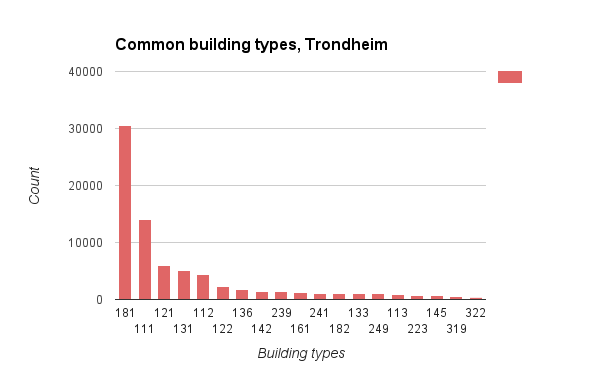
\includegraphics[scale=0.6]{figures/FixedByMe/buildtypestrd.png}
    \caption{20 most common building types in Trondheim, see table \ref{tab:fkbtoosmdel1} for building type conversion. Source: postgis query in the cadastre} 
    \label{fig:buildtypTrd}
\end{figure}

The values in table \ref{tab:fkbtoosmdel1} and \ref{tab:fkbtoosmdel2} will represent the value for the building key. This information will, as mentioned , be added to the building outline. For the different feature types introduced in section \ref{sec:FKBbuilding} there are different approaches to how they should be conveted to OSM. Using section \ref{sec:FKBbuilding} and figure \ref{fig:ridgeedge} the main feature types can be given the key-value pairs shown in table \ref{tab:featuretypesinOSM}. More about this in section \ref{sec:3D_OSM}.

\begin{table}[H]
\begin{tabular}{ | l | l | l | }
\hline
	FKB: feature type & Key & Value \\ \hline
	Roof edge (\textit{Takkant}) & building & yes \\ \hline
	Ridge line (\textit{Mønelinje}) & roof:ridge & yes \\ \hline
	Building line (\textit{bygningslinje}) & roof:edge & yes \\ \hline
	Roof overhang (\textit{Taksprang}) & roof:edge & yes \\ \hline
	Roof overhang bottom (\textit{TaksprangBunn}) & roof:edge & yes \\ \hline
\end{tabular}
\caption{Translating FKB feature types to OpenStreetMap key-value pairs}
\label{tab:featuretypesinOSM}
\end{table}

\section{Conversion using existing script}\label{sec:sosi2osm}
% fkbbuilding.lua
%Lage utkast til en luafil, vise hvordan xml oppsettet blir 
Before implementing a new script to convert the FKB SOSI files to OSM XML-files, existing scripts should be evaluated. There are at least one script that converts SOSI files to OSM XML-files. This script was used by the N50 import team. The script is called sosi2osm and was developed in 2013 by the github user Gnonthgol.
 The script is open source and the repository is available at Gnonthgol's GitHub account. The sosi2osm repository do not have any documentation, the only available help is a wiki page who shortly explain how to install and run the code. It is very difficult to install, especially if you don't have a linux operating system. 
 
The script depends on fyba. An open source code distributed by the National Mapping Authority of Norway (Kartverket) to read and write SOSI files. Sosi2osm do not support SOSI files encoded in UTF-8. This is a challenge since FKB sosi files can be UTF-8 encoded.*%Er FKB alltid UTF8 eller bare i noen kommuner?
 This is a major drawback with this script. To test the script, after managing to install it correctly, the first step is to encode the FKB SOSI file into ISO8859-10. This step should not have been necessary.  %Er alle SOSI filer i UTF 8 idag?

When running the script the input is a sosi file and a lua script. A new lua script needs to be created for every new dataset. The lua script needs to fit the metadata present in the dataset the user is converting. In the N50 import they created a lua script for land cover (\textit{arealdekke}) without water and one lua script for only water \cite{OpenStreetMapn}. The lua script creates key-value pairs from the metadata of the input file. Important metadata in SOSI files is the feature type (\textit{OBJTYPE}). In FKB building files, another important attribute is $BYGGTYP\_NBR$ which give information of what kind of building it is, introduced in the previous section. 

To test the sosi2osm script on the FKB building dataset a fkbbuilding.lua file was created. Using only the most common feature type in the dataset shown in figure \ref{fig:commfeattypes}. Adding values to the building key, which depend on the buildingtype code in FKB,  table \ref{tab:fkbtoosmdel1} and \ref{tab:fkbtoosmdel2} was used. See listing \ref{eq:luabuldtype} in the appendix for a code snip from the lua script checking the building value. This code snip checks the $BYGGTYP\_NBR$ attribute value to determine the buildings particular usage. The building=* key-value pair will be placed on the buildings footprint, since only building feature in FKB has the $BYGGTYP\_NBR$ attribute value. 

A problem with the sosi2osm script is that it is not possible to retrieve height data from the SOSI file. It is then not possible to use this script to create 3D models. It do not consider height values, creating one node for each north, east coordinate pair. If two crossing building lines have different height values they should not share the same node \cite{OpenStreetMap2015}. This is also a problem, especially when considering 3D modeling of buildings. More about this in section \ref{sec:3D_OSM}. 

The resulting OSM XML-file created by the sosi2osm script made an functional representation of building outlines with the roof lines. The output file was tested using the JOSM editor. Test buildings was withdrawn from the scripts output osm file and then imported into JOSM for testing. The conversion worked in creating the building outline with the roof lines, shown in figure \ref{fig:2d_sosi2osm}. The key-value pairs was set correctly and a representation tag was created for the building outline.  

\begin{figure}[H]
\centering
\begin{subfigure}{.5\textwidth}
    \centering
    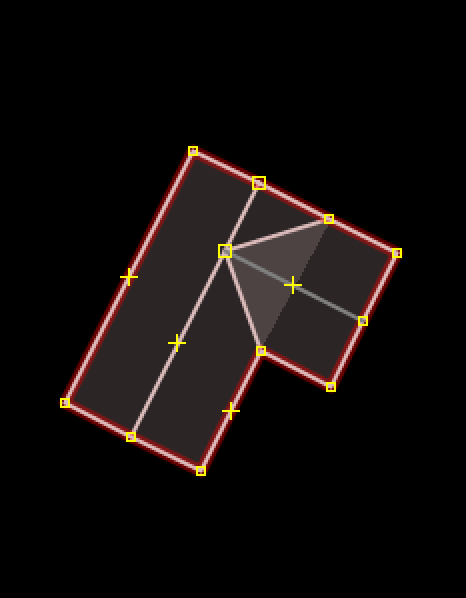
\includegraphics[scale=0.6]{figures/FixedByMe/2Doutlinesosi2osm.png}
    \caption{Building footprint 1} 
    \label{fig:2D2}
\end{subfigure}%
\begin{subfigure}{.5\textwidth}
    \centering
    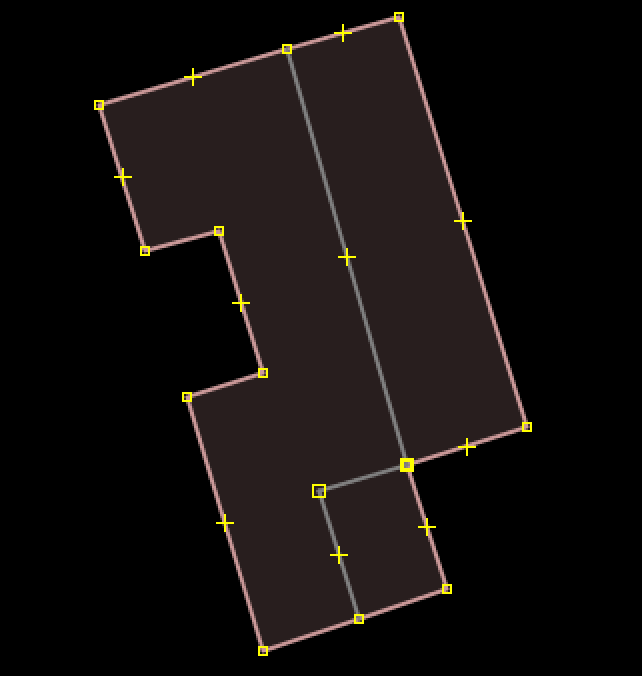
\includegraphics[scale=0.5]{figures/FixedByMe/2Doutline.png}
    \caption{Building footprint 2} 
    \label{fig:2D1}
\end{subfigure}
\caption{Building footprint with roof edges and roof ridges created with sosi2osm script}
\label{fig:2d_sosi2osm}
\end{figure}


\section{How to map FKB buildings in 3D}\label{sec:3D_OSM}
%Her kan jeg lage et eksempel på hvordan 3D bygg kan moduleres i OSM XML format. 
In order to create a XML representation capable of modeling FKB buildings in 3D, a standard approach should be developed. Members of the OpenStreetMap community, with interest in 3D mapping, started in March 2012 to unite all the separated approaches to model 3D buildings using OSM XML \cite{OpenStreetMapm}. They arranged workshops, which resulted in a suggestion for a simple 3D building schema. This is the approach mentioned in section \ref{buildOSM}. This approach is fairly easy to implement, if the building's roof shape is known. This is not the case for the FKB buildings, so the simple 3D building schema needs modifications.

\begin{figure}[H]
\centering
\begin{subfigure}{.5\textwidth}
    \centering
    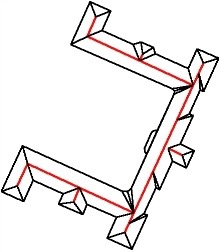
\includegraphics[scale=0.6]{figures/FixedByMe/roof-ridges}
    \caption{Roof ridges} 
    \label{fig:roofridge}
\end{subfigure}%
\begin{subfigure}{.5\textwidth}
    \centering
    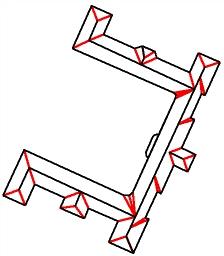
\includegraphics[scale=0.6]{figures/FixedByMe/roof-edges}
    \caption{Roof edges} 
    \label{fig:roofedge}
\end{subfigure}
\caption{Roof lines in OpenStreetMap, source: \cite{OpenStreetMapo}}
\label{fig:ridgeedge}
\end{figure}

Buildings in FKB is modelled with ridge and edge lines and they can be used to create 3D models, see the figures in section \ref{sec:FKBbuilding}. When using ridge and edge modeling, roof shape tags are ignored \cite{OpenStreetMap2015a}, meaning the shape of the roof is not needed. Using figure \ref{fig:ridgeedge} as guidance. Ridge- and edge-lines for one building was collected to test this method and manually created a way-representation for each line with roof:edge and roof:ridge key's. The key-value pairs for each roof feature line is shown in table \ref{tab:featuretypesinOSM}. The way-tag representing the building outline, which is most often the roof-edge (\textit{takkant}) feature as mentioned in section \ref{sec:FKBbuilding}, must hold the building=yes, height and roof:height information.*%Funker ikke paa alle type bygninger, bare de som har en closed-way rundt hele omrisset
This of course only works on buildings where the whole building outline is only covered by the roof edge, this is not always the case. 

Listing \ref{eq:3D_fkbbuilding} in the appendix creates a 3D representation of a house in OSM from FKB data using the method described above. The house is shown in figure \ref{fig:3DFKBbuild}, using the JOSM editor to generate the code in listing \ref{eq:3D_fkbbuilding} and getting 3D visualization using the JSOM plugin kendzi3d. The building outline in this building is only covered by the roof edge, meaning it's SOSI area representation only refers to one roof edge. The area representation of the building in figure \ref{fig:3DFKBbuild} in SOSI format is shown in listing \ref{eq:buildingfootpr}, notice that it only refers to one feature type (REF :166806). The feature with id=166806 is a roof edge. Then the technique described above works. 

\begin{figure}[H]
    \centering
    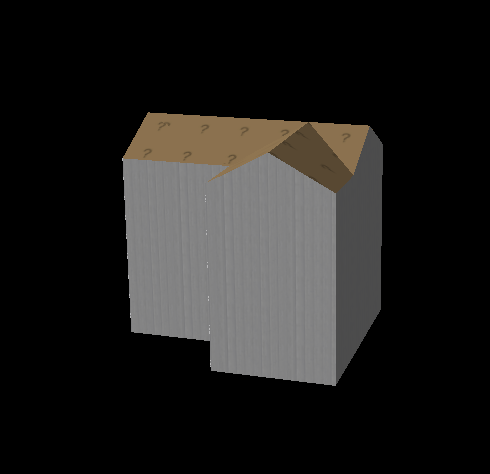
\includegraphics[scale=0.5]{figures/FixedByMe/3DFKBbuilding.png}
    \caption{3D representation of a FKB building, result of listing \ref{eq:3D_fkbbuilding}}
    \label{fig:3DFKBbuild}
\end{figure}

Getting the method working for buildings referring to more than one feature is more challenging, especially when the goal is to create a script that creates a working 3D model for every building type. A solution could be to gather all the features the building refers to in the SOSI file and join then in one way representation in OSM XML. This was tested manually, and it worked for the test objects. It's of course difficult to test every different case. Fining an approach that can manage every building type will take time.

Getting the height of the buildings correct is also a challenge. In OpenStreetMap, building height is the distance between the lowest possible position with ground contact and the top of the roof of the building, excluding antennas, etc \cite{OSMwikipage2016}. Height of buildings in FKB is height above sea level.  In listing \ref{eq:3D_fkbbuilding} height above sea level is manually withdrawn from the height given from the FKB data. A solution is to use a digital elevation model to examine the elevation at every building. This will of course again cause challenges, for instance if a house is built into a hillside. Solving this is outside the scope of this study, but is important to look into if/when an import of FKB building data is on the agenda. 

Another problem that arose when testing 3D modeling in OSM is overlapping nodes with different heights. The problem with not distinguishing between overlapping nodes with different heights, mentioned in section \ref{sec:sosi2osm}, make 3D modeling of buildings with overlapping roof ridges and edges a challenge. This problem is shown in figure \ref{fig:3DFKBbuildFail} and how the building actually should have been modelled is shown in figure \ref{fig:3DFKBbuildFail2}. Here it's easy to see the effect of overlapping points, they should be located in different heights, but share nodes when using the sosi2osm script.  This is something to consider if/when a new conversion script is implemented. 

\begin{figure}[H]
\centering
\begin{subfigure}{.5\textwidth}
    \centering
    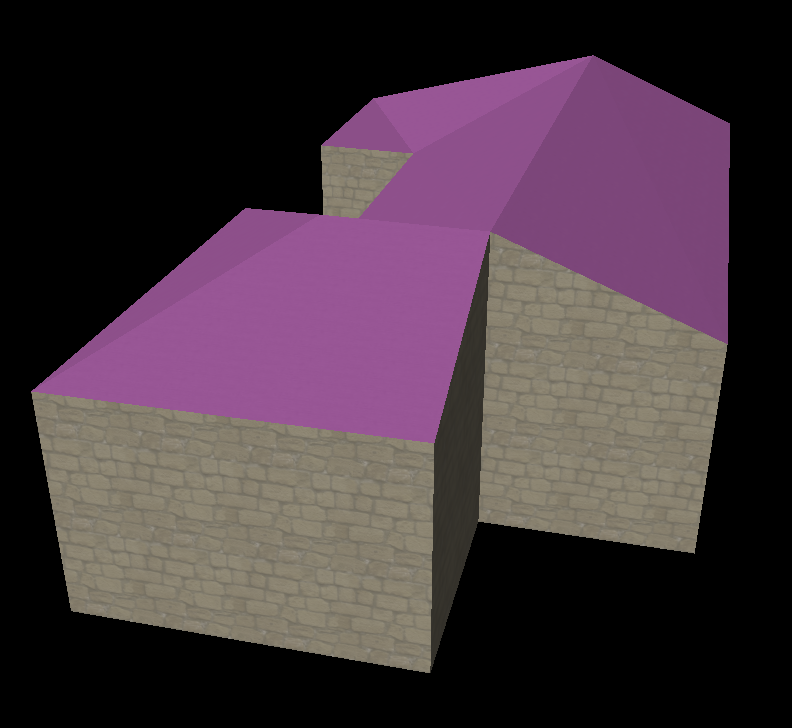
\includegraphics[scale=0.4]{figures/FixedByMe/samenode_but_have_diff_height.png}
    \caption{Building who share nodes placed at the same position but have different heights}
    \label{fig:3DFKBbuildFail}
\end{subfigure}%
\begin{subfigure}{.5\textwidth}
  \centering
  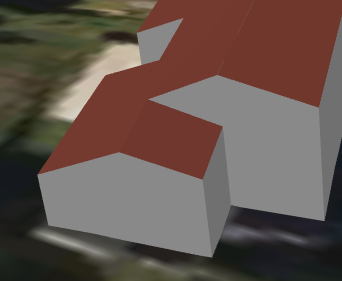
\includegraphics[width=0.8\linewidth]{figures/FixedByMe/112building_nodes_with_diff_height.png}
  \caption{Building in 3d.kommunekart.com}
  \label{fig:3DFKBbuildFail2}
\end{subfigure}
\caption{3D representation of a FKB building, showing the problem with overlapping points with different heights in OSM}
\label{fig:3dfail}
\end{figure}

%There are different tools developed to visualizing 3D buildings with data from OSM. A problem is that not all tools supports the different modelling. A list of which of them who supports the simple 3D building schema is located at the OSM simple 3D buildings wiki page, most tools accept this schema. 7 tools supports building:part=yes. %http://wiki.openstreetmap.org/wiki/3D_Development/Tagging#Usage_Community
\chapter{Discussion}
The findings in this study show how the FKB building data could be imported into OpenStreetMap, both which method to use and technical challenges and suggestions. The micro-tasking method is the suggested method for this study, and by evaluating both other import methods but also imports who used this method try to conclude if this is the preferred method. This study hopefully also present good arguments in favor of importing FKB data into OSM. 

Why import the FKB data? The FKB data is more detailed and accurate than for instance the TIGER data, and also more accurate than N50 data. The accuracy of FKB building data varies from +/- 0.20 m to +/- 2 m, depending on the FKB standard covered in the area the building lies in, as introduced in section \ref{sec:FKB_quality}. The N50 data is adapted to a scale range of 1:25000 to 1:100000 \cite{Geonorge}, while FKB is adapted to a scale range of 1:5000 to 1:30000 \cite{Geonorge2014}. The FKB data, especially the building data, can raise the quality of the OSM-map. Increasing the quality of data in OSM can increase the usage of the map. The community wants the map to be used, and if this can contribute to increased usage, the import will contribute in a positive manner. There will always be people negative to such an import, and there are good arguments on both sides. This study chose to see the arguments in favor of this import, especially if it results in a 3D model of all buildings in Norway. A free and open solution with a 3D model of all buildings in Norway will, with little doubt, increase the popularity of OpenStreetMap, especially among the Norwegian people.

From the beginning of the New York building import, a goal was to help the city government maintain its building and address datasets \cite{Barth2014b}.  An edit in OSM can be a signal that the building has changed or the imported data is wrong. The solution was to offer the New York GIS department a subscription to daily email notifications on building and address changes in OSM. An excellent example of how government and open source *%Riktig m open source her?
  can take advantage of each other. Such a collaboration could also be evaluated and discussed if/when an FKB import is approved. Another argument in favor of importing the FKB building dataset into OSM. 
  
This paper only provides an overview study of how FKB buildings could be 3D modeled in OpenStreetMap. More time needs to be spent investigating possible methods. It is not certain that it's possible to find a uniform method for all building types. This study can't answer that. Further studies must be conducted to be able to evaluate how to model different building types and also evaluate different 3D modeling schemas supported by OpenStreetMap.

\chapter{Conclusion}
Results of this study show that micro-tasking can be a suitable method if/when importing the FKB datasets into OpenStreetMap. Two building imports, in New York and Los Angeles, already tried the method and both imports was successful. 